\subsubsection{Representation}
\label{sec:bg:gp:repr_ev:repr}
  As with GAs, the representation of the individuals is one of the most 
  important aspects of GP.
  The representation is the encoding of potential solutions to the problem into
  a form that can be manipulated,\footnote{
    For example, by applying genetic operators.
  } executed and evaluated by the algorithm.

  Various methods exist for program representation, such as utilizing an 
  abstract syntax tree, a linear sequence of instructions, a stack of 
  instructions, or a combination of these approaches.
  However, the most classical representation is the \emph{tree representation}, 
  where the program is represented as a composite data structure like the one 
  shown in the introduction to this section.

  Let's illustrate this with an example problem: given a set of \(n\) points in
  the plane, find the curve that best fits the points.
  This is a very common problem in statistics, and it is known as the
  \emph{symbolic regression} 
  problem~\autocite{kozaGeneticProgrammingProgramming1992a}.
  In this example, our goal is to use symbolic regression to approximate the 
  function

  \begin{equation}
    f(x) = 5x^3 - 2x^2 + \sin(x) - 7;\; x \in [-1, 1]
  \end{equation}

  using this function, we can generate a set of points that lies on the curve as
  shown in \vref{fig:bg:gp:repr_ev:points} and 
  \vref{tab:bg:gp:repr_ev:points}.

  The next step in preparing our GP setup is to define the primitive set, which
  includes the functions and terminals that the algorithm can use to construct
  candidate solutions.
  In this case, we will use the following set of functions and terminals:

  \begin{itemize}
    \item \textbf{Functions:}
      \begin{enumerate*}
        \item \(+\) (Addition)
        \item \(-\) (Subtraction)
        \item \(\times\) (Multiplication)
        \item \(/\) (Division)
        \item \(\sin\) (Sine)
        \item \(\cos\) (Cosine)
        \item \(\mathrm{pow}\) (Power)
      \end{enumerate*}
    \item \textbf{Terminals:}
      \begin{enumerate*}
        \item \(x\) (The variable \(x\))
        \item \(\{c\ |\ c \in [1,\, 7] \wedge c \in \mathbb{Z}\}\) (An ephemeral
          constant)\footnote{See \vref{def:ephemeral_constant}.}
      \end{enumerate*}
  \end{itemize}

  \begin{figure}[ht!]
    \centering
    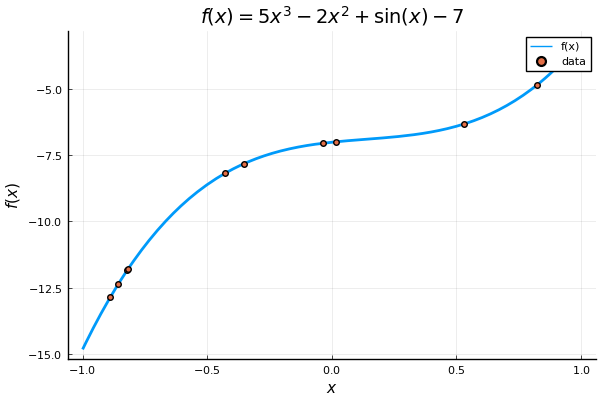
\includegraphics[width=0.6\textwidth]{img/theoretical_framework/symbolic.png}
    \caption{
      A set of points generated from the function \(5x^3 - 2x^2 + \sin(x) - 7\)
    }
    \label{fig:bg:gp:repr_ev:points}
  \end{figure}

  \subimport{./}{tab-bg-gp-repr_ev-points.tex}

  Using this set of functions and terminals, we can represent the program as a
  tree, as shown in \vref{fig:bg:gp:repr_ev:tree}.

  \begin{figure}[ht!]
    \centering
    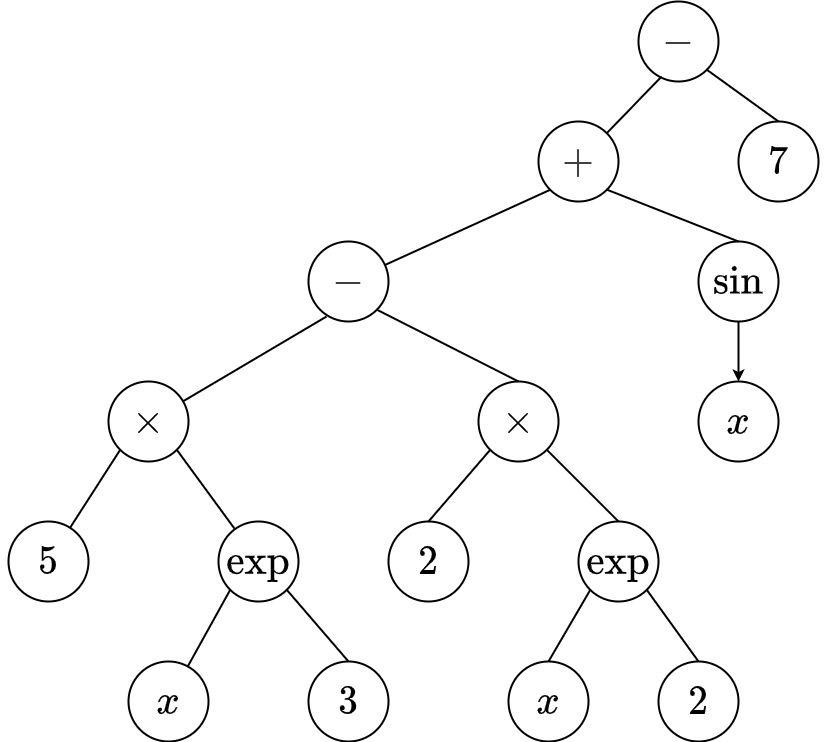
\includegraphics[width=0.4875\textwidth]{img/theoretical_framework/Expected Expression Tree.png}
    \caption{
      A possible tree representation of the program \(5x^3 - 2x^2 + \sin(x) - 7\)
    }
    \label{fig:bg:gp:repr_ev:tree}
  \end{figure}

  Note that this definition arises the possibility of having a program that
  has an infinite number of nodes, as the tree can grow indefinitely.
  This leads the search to be unsuccessful since the probability of finding a
  solution is close to zero, for example, the probability of finding a solution
  on the initial population would be: \(\lim_{x \to \infty} \frac{1}{x} = 0\).
  To avoid this issue of potentially infinite trees, we typically impose certain
  \emph{constraints} on the generation of the trees.
  The most common constraints are the \emph{maximum height} of the tree and the
  \emph{maximum number of nodes} in the tree.
